% Originally: content/week-02.tex, \section{Open and closed sets} (Corsin Week 2, Monday)

% Retitled from "Open and closed sets" now that the chapter carries that name; the label is
% unchanged, so every existing \cref still resolves.
\section{Open balls, open and closed sets}
\label{sec:open_closed_sets}

\begin{definition}[Open ball]
\label{def:open_ball}
Let $(X,d)$ be a metric space, let $x \in X$, and let $r \in \mathbb{R}$. Then we define the
\newterm{open ball} of radius $r$ as
\[B_r(x) := \{\,\boxed{y \in X}\, : d(y,x) < r\,\}\]
\end{definition}

\begin{importantremark}
Corsin marks the boxed part in red as an \qt{important subtlety}: the ambient set $X$ in
$y \in X$ is what makes openness relative to the space, and it is exactly what the common
misconception on \cref{rem:common_misconception} turns on.
\end{importantremark}

\begin{ainote}
\Cref{def:open_ball} is stated for $r \in \mathbb{R}$ rather than $r > 0$. Harmless here, but
loose.
\end{ainote}

% Moved here from before \cref{def:open_ball} (review item D1): it uses $B_r(x)$,
% "open" and "clopen", none of which were defined at its former position.
\begin{aiexample}[Open Balls in the Discrete Metric]
% Generator: Gemini 3.6 Flash (Medium)
Let $(X, d_{\text{disc}})$ be a discrete metric space. The open ball $B_r(x)$ centered at
$x \in X$ with radius $r > 0$ is
\[
B_r(x) = \begin{cases} \{x\} & \text{if } 0 < r \leq 1, \\ X & \text{if } r > 1. \end{cases}
\]
Hence every singleton $\{x\}$ is open in the discrete metric, and consequently every subset of
$X$ is both open and closed (\newterm{clopen}). This is exactly what \Cref{ex:X_empty_clopen}
below asks you to verify for $X$ and $\emptyset$ in a general metric space.
\end{aiexample}

% Generator: Claude Opus 5 (Medium)
\begin{remark}[Two degenerate balls worth knowing]
Taking \cref{def:open_ball} literally at the edges of its range is a cheap way to test whether
you have read it correctly.
\begin{itemize}
  \item If $r \leq 0$, then $B_r(x) = \emptyset$, and \emph{not} $\{x\}$. The condition is
    $d(y,x) < r$, strictly, and $d(x,x) = 0 \not< 0$. So even the centre is missing from
    $B_0(x)$.
  \item In the discrete metric $B_1(x) = \{x\}$, while $B_{1.01}(x) = X$: a ball can jump from a
    single point to the entire space without passing through anything in between. Radii do not
    have to behave like radii.
\end{itemize}
These are the two cases that make \qt{shrink the ball a little} arguments go wrong if applied
without thinking.
\end{remark}

% Generator: Claude Opus 5 (Medium)
\begin{aiexercise}[Open balls are open]
\label{ex:ai_open_balls_are_open}
The name promises it, but \cref{def:open_ball} does not say it. Show that in any metric space
$(X,d)$ the ball $B_r(x)$ is an open set in the sense of \cref{def:open_closed}.

\textit{Hint:} given $y \in B_r(x)$, the number $\varepsilon := r - d(y,x)$ is strictly positive.
Draw the picture, then let the triangle inequality do the work.
\end{aiexercise}

\begin{definition}[Open and closed sets]
\label{def:open_closed}
Then, we call a subset $U \subseteq X$ \newterm{open} (\germanterm{offen}) if and only if
\[\forall y \in U \ \exists \varepsilon > 0 \text{ such that } B_\varepsilon(y) \subseteq U.\]
And we call $A \subseteq X$ \newterm{closed} (\germanterm{abgeschlossen}) if and only if
$X \setminus A$ is open.
\end{definition}

\begin{center}
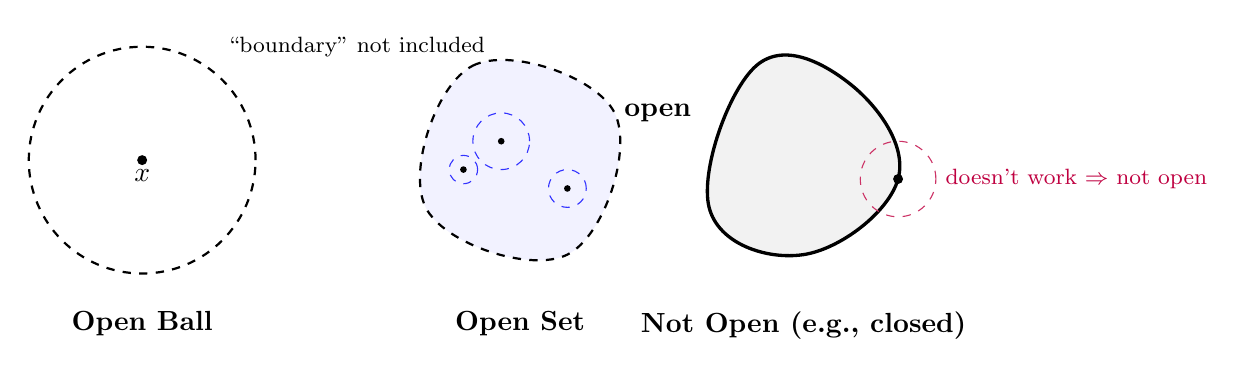
\begin{tikzpicture}[scale=1.2]
  % Open Ball
  \draw[dashed, thick] (0,0) circle (1.2);
  \fill (0,0) circle (1.5pt) node[below] {$x$};
  \node[anchor=west] at (0.8, 1.2) {\footnotesize ``boundary'' not included};
  \node[below] at (0, -1.5) {\textbf{Open Ball}};

  % Open set
  \begin{scope}[xshift=4cm]
    \draw[dashed, thick, fill=blue!5] 
      plot[smooth cycle, tension=0.7] coordinates {(-1,-0.5) (-0.5,1) (1,0.5) (0.5,-1)};
    \fill (-0.2,0.2) circle (1pt);
    \draw[dashed, blue!80] (-0.2,0.2) circle (0.3);
    \fill (0.5,-0.3) circle (1pt);
    \draw[dashed, blue!80] (0.5,-0.3) circle (0.2);
    \fill (-0.6,-0.1) circle (1pt);
    \draw[dashed, blue!80] (-0.6,-0.1) circle (0.15);
    \node[right, font=\bfseries] at (1, 0.5) {open};
    \node[below] at (0, -1.5) {\textbf{Open Set}};
  \end{scope}

  % Not Open set (Closed / boundary included)
  \begin{scope}[xshift=7cm]
    \draw[very thick, fill=gray!10] 
      plot[smooth cycle, tension=0.7] coordinates {(-1,-0.5) (-0.5,1) (0.5,0.8) (1,-0.2) (0,-1)};
    \fill (1,-0.2) circle (1.5pt);
    \draw[dashed, purple!80] (1,-0.2) circle (0.4);
    \node[purple, right] at (1.4, -0.2) {\footnotesize doesn't work $\Rightarrow$ not open};
    \node[below] at (0, -1.5) {\textbf{Not Open (e.g., closed)}};
  \end{scope}
\end{tikzpicture}
\end{center}

% Supplement: Analysis_II_Script_v1.pdf, p. 14
\begin{example}[Clopen sets other than $X$ and $\emptyset$]
\label{ex:clopen_nontrivial}
\Cref{ex:X_empty_clopen} shows $X$ and $\emptyset$ are always clopen, but nothing in
\cref{def:open_closed} forces these to be the \emph{only} clopen subsets of $X$. Take
$X := (0,1)\cup(2,3) \subset \mathbb{R}$ with the standard metric: both $(0,1)$ and $(2,3)$ are
clopen \emph{in $X$}. Each is open in $\mathbb{R}$, hence open in $X$; and each is the complement
in $X$ of the other, so each is also closed in $X$. Whether a space has clopen subsets besides
$X$ and $\emptyset$ turns out to be exactly the question \cref{ch:connectedness} is organised
around. A space with none is called \newterm{connected}.
\end{example}

% Supplement: Sascha Brack/Class Notes/Week_02_Notes_Friday_Updated.pdf, p. 1
\begin{proposition}[How open and closed sets combine]
\label{prop:open_closed_operations}
Let $(X,d)$ be a metric space.
\begin{enumerate}[label=\textbf{(\alph*)}]
  \item \label{item:arbitrary_union_open}
    \textbf{Arbitrary} unions of open sets are open: if $\{U_i\}_{i \in I}$ are open, so is
    $\bigcup_{i\in I}U_i$.
  \item \label{item:finite_intersection_open}
    \textbf{Finite} intersections of open sets are open: if $U_1,\dots,U_k$ are open, so is
    $\bigcap_{i=1}^{k}U_i$.
  \item \textbf{Arbitrary} intersections of closed sets are closed, and \textbf{finite} unions
    of closed sets are closed.
\end{enumerate}
\end{proposition}

\begin{proof}
\textbf{(a)} Let $x \in \bigcup_i U_i$. Then $x \in U_{i_0}$ for some $i_0$, and since $U_{i_0}$
is open there is $\varepsilon>0$ with $B_\varepsilon(x) \subseteq U_{i_0} \subseteq \bigcup_iU_i$.

\textbf{(b)} Let $x \in \bigcap_{i=1}^kU_i$. For each $i$ pick $\varepsilon_i>0$ with
$B_{\varepsilon_i}(x) \subseteq U_i$, and set $\varepsilon := \min\{\varepsilon_1,\dots,\varepsilon_k\}$.
Then $\varepsilon > 0$, and \emph{this is the only place finiteness is used}: a minimum of
finitely many positive numbers is positive, whereas an infimum of infinitely many can be $0$.
Since $B_\varepsilon(x) \subseteq U_i$ for every $i$, we conclude that
$B_\varepsilon(x) \subseteq \bigcap_iU_i$.

\textbf{(c)} Take complements and apply \textbf{(a)}, \textbf{(b)} via De Morgan:
$X\setminus\bigcap_iA_i = \bigcup_i(X\setminus A_i)$ and
$X\setminus\bigcup_{i=1}^kA_i = \bigcap_{i=1}^k(X\setminus A_i)$.
\end{proof}

% Generator: Claude Opus 5 (Medium)
\begin{importantremark}[The asymmetry is real, not an artefact of the proof]
\label{rem:finiteness_is_necessary}
It is tempting to read \qt{finite} in \textbf{(b)} as laziness. It is not: an infinite
intersection of open sets genuinely need not be open. In $\mathbb{R}$,
\[\bigcap_{n=1}^{\infty}\left(-\tfrac1n,\ \tfrac1n\right) = \{0\},\]
an intersection of open intervals which is not open. The proof shows exactly where it breaks:
$\varepsilon := \min_i\varepsilon_i$ is the whole argument, and an infimum of infinitely many
positive numbers can be $0$. Dually, $\bigcup_{n\geq1}\big[\tfrac1n,1\big] = (0,1]$ is an
infinite union of closed sets that is not closed.

\begin{ainote}
These four closure properties are exactly the axioms of a \newterm{topology}, which is how the
subject is set up when one drops the metric altogether (\cref{sec:structured_spaces},
\qt{fourth semester}). That is why they are worth isolating: they are the only facts about open
sets that survive into the general theory.
\end{ainote}
\end{importantremark}

% Supplement: Sascha Brack/Class Notes/Week_02_Notes_Friday_Updated.pdf, p. 1
\begin{example}[Open and closed sets in $\mathbb{R}$]
\label{ex:open_closed_R}
Consider the following subsets of $\mathbb{R}$ with the standard metric:
\begin{enumerate}[label=\textbf{(\alph*)}]
  \item \textbf{Is $\mathbb{N}$ open, closed, or neither?} It is \textbf{closed}, since its
    complement $\mathbb{R} \setminus \mathbb{N} = (-\infty, 1) \cup \bigcup_{n=1}^\infty (n, n+1)$
    is a union of open intervals, which is open by
    \Cref{prop:open_closed_operations}\textbf{\ref{item:arbitrary_union_open}}. It is not open,
    because no open ball around any $n \in \mathbb{N}$ is contained in $\mathbb{N}$.
  \item \textbf{Let $A := \{\frac{1}{n} \mid n = 1, 2, \dots\}$.} The set $A$ is \textbf{neither}
    open nor closed. It is not open for the same reason as $\mathbb{N}$. It is not closed because
    $0$ is an accumulation point of $A$, but $0 \notin A$, meaning its complement
    $\mathbb{R} \setminus A$ is not open (any open ball around $0$ intersects $A$).
  \item \textbf{Let $F := \{\frac{1}{n} \mid n = 1, 2, \dots\} \cup \{0\}$.} The set $F$ is
    \textbf{closed}. By adding the limit point $0$, the complement $\mathbb{R} \setminus F$
    becomes a union of open intervals, which is open.
\end{enumerate}
\end{example}

% Supplement: Linus Lüchinger/Slides/Slides-02-23.pdf, slide 20
% Linus's self-test list. The three entries Sascha already works above (N, {1/n},
% {1/n} u {0}) are dropped; what remains is the part that is not already answered.
\begin{exercise}[A longer self-test]
\label{ex:open_closed_self_test}
Linus sets the following list as a self-test at the end of his first session. Each subset of
$\mathbb{R}$ carries the standard metric; decide for each whether it is \textbf{open},
\textbf{closed}, \textbf{both}, or \textbf{neither}.
\begin{enumerate}[label=\textbf{(\alph*)}]
  \item $[0,\infty)$
  \item $\mathbb{Q}$
  \item $\{x - \lfloor x \rfloor : x \in \mathbb{R}\}$
  \item $S := \{x \in \mathbb{R} : x\cdot 2^p \in [1,2] \text{ for some integer } p \geq 0\}$
  \item $T := \{x \in \mathbb{R} : x\cdot 2^p \in (1,2) \text{ for some integer } p \geq 0\}$
  \item $\{x_n : n \in \mathbb{N}\}$, where $x_0 := 1$ and
    $x_n := \tfrac12\big(x_{n-1} + x_{n-1}^2\big)$
  \item $\{\Rea(c) : c \in \mathbb{C},\ \zeta(c) = 0\}$, where $\zeta$ is the Riemann zeta
    function
\end{enumerate}
Compare \textbf{(d)} with \textbf{(e)} before reading the solution: the two differ only in one
bracket.
\end{exercise}

% Quelle: Jérôme Paschoud/Notizen/Woche 2.1 Metrische Räume.pdf, p. 5
\begin{exercise}[Relative openness]
\label{ex:relative_openness_subsets}
Let $X := (\{0\} \times \mathbb{R}) \cup (0,1)^2$ be equipped with the subspace metric from $\mathbb{R}^2$. Consider the following subsets of $X$:
\begin{align*}
  A &:= \{(x,y) \in \mathbb{R}^2 \mid x = 0, y \in (2,3)\} \\
  B &:= \left\{(x,y) \in \mathbb{R}^2 \ \middle|\ \left(x - \tfrac12\right)^2 + \left(y - \tfrac12\right)^2 < \tfrac{1}{16}\right\}
\end{align*}
Are $A$ and $B$ open with respect to $X$? Are they open with respect to $\mathbb{R}^2$?
\end{exercise}

% Generator: Gemini 3.6 Pro
\begin{exercisesolution}[Proof of \cref{ex:relative_openness_subsets}]
\begin{itemize}
  \item $A$ is \textbf{open with respect to $X$}, but \textbf{not open with respect to $\mathbb{R}^2$}. It is open in $X$ because $A = X \cap U$ where $U = (-\varepsilon, \varepsilon) \times (2,3)$ is an open set in $\mathbb{R}^2$. It is not open in $\mathbb{R}^2$ because any open ball around a point in $A$ will contain points with $x \neq 0$, which are not in $A$.
  \item $B$ is \textbf{open with respect to both $X$ and $\mathbb{R}^2$}. $B$ is exactly the open ball $B_{1/4}((\tfrac12, \tfrac12))$ in $\mathbb{R}^2$, which is open in $\mathbb{R}^2$. Since $B \subseteq (0,1)^2 \subset X$, we have $B = X \cap B$, so $B$ is also open relative to $X$.
\end{itemize}
\end{exercisesolution}
